\chapter{Conclusions}

Only a few months might not sound much but is enough to obtain some
conclusion about techonologíes, patterns and ways to develop.

\begin{flushleft}
This work can not finish without a reflexion about what have been the mainly
drawbacks and locks in the develop, design and evolution of the entire project,
trying to propose solutions and overall, learning a lot about all.
\end{flushleft}

\subsection{Scheduling}

The scheduling of development is very easy to do, in the hypothetical case that
all goes fine, but as is normal, there are a lot of factors hard to control that
besides are unknown at the beginning.
If we join this with an inexpert scrum master and technologies absolutely new for
the team (without a good spikes issues to select and try these) the result can
be catastrophic.
Despite this, the result is not as wrong as could be,
and with all predictable fails, it has not been a bad finish.

\subsection{Technologies and frameworks}

Of one side, we have the difficulties with the technology choice. In this case
can be said that use AngularJS and Python has been literally perfect, beyond
that the typical novice errors with the languages and their learning curves.
So, in general, without a doubt, they will be chosen as technologies again.
\linebreak
\linebreak
\noindent About the platforms or technologies the point of view changes. If you are
really expert developer using platforms like Google App Engine can be really
interesting, because you are evaluated the rest of the options, but when
you don't have any practice, in my view, is not a good option. Moreover when
the learning curve is so soft.

\noindent As in many new technologies is easy do the first steps, but develop some bigger
is another thing, specially when we are not talking about frameworks and
languages standard as C++, Java or PHP. So, before to select one is rellay justify
the spike of some of these.

\noindent About the API frameworks, Flask was a good selection, because their ease of use
and lightness does it perfectly. However, when we analyze the performance, there are
other solutions also in python faster. An example of this is Falcon\footnote{Defined as: \textit{"A
very fast, very minimal Python web framework for building microservices, app backends,
and higher-level frameworks"}. More info at: \textit{falconframework.org}}. As can be
seen in the next picture, extracted from py-frameworks-bench\footnote{
http://klen.github.io/py-frameworks-bench/} project, we can see how Falcon has
better performance than Flask. In this grapihc is measure the response in ms
of encode a object to JSON and return the response.

\begin{center}
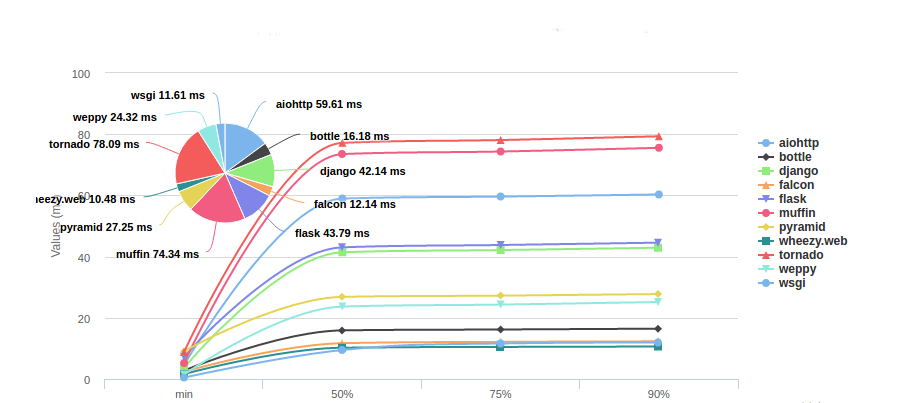
\includegraphics[scale=0.5]{img/graphics/frameworks.png}
\end{center}

\noindent And Falcon would be our selection today (even more having some practice in
company).
\linebreak
\linebreak
\noindent About Sphinx, is a good choice, but it has something that could be improved and
is the requirements of that the project must have. To use Sphinx your project
needs to be \textit{executable}, understanding this as all imports must work.
Many people do not know why Sphinx have this restriction, so if you
only want doc, independently of if you structure is correct or not, well, this is
impossible in the actual version, we hope that change this at any moment.

\subsubsection{About the platform}

In spite of Google App Engine is a good tool it has some drawbacks that some are
very obvious at first and others that can go unnoticed until you are working with it.
the sandbox restrictions as use python only in their version 2.7 at first is not
a problem but when you discover that the most of libraries that you need works
better in 3.x, or some are deprecated in 2.7, out of maintenance is not a good
signal, specially when you have some block and the help of community is focused
on upper versions. It happened in the standar version of App Engine sandbox, to
solve this the team of it launched App Engine Flexible Environment, where you can
run any code but the configuration is not trivial and although is configurable by
dockerfile is a strange mixin between the automainteined and scalables isolated
sandboxs and the clasic containers developer managed.
\linebreak
\linebreak
\noindent So, taking advantage of all services of the infrastructure of GCE, another
architecture that we will develop in the future will run only into docker containers,
using the services required (SQL, DataStore or another and runing over compute layer,
not with google app engine.

\subsubsection{About the database}

About database, without doubt MongoDB is nowadays the better solution that
can be used in a project with low relational requirements, because their learning
curve is so good that is easy to have a good prototipe of database layer soon,
and the resources of the community is greatly assist.

\subsection {Design}

\subsubsection{About the user interface}

There are any that has been critical in the develop and is that the assumption
as a good idea that all interface always is loaded when a user enters to the app,
but after some tests have been seen that is not the best way.  For this reason,
many teams that work with Angular choose an alternative, use a library specially
designed to load the javascript files of the app needed in each part of the interface.
So, if a user is in the teaching section don't need all files of the reports section
and this files only will be loaded when the user insert in this section. To do this,
the teams use the Require.js\footnote{Literraly from their website ,requirejs.org: \textit{"RequireJS is a
JavaScript file and module loader. It will improve the speed and quality of your code."}} library as
the standard dynamically loader and their use will be the next step to do the
load of the app faster.

\subsubsection{About the compression of APIs}

Is easy to notice that the API of Students Control microService is very semantic
but very big also (become more complex to maintain and change) while of the
teaching service API is very compact and little but less semantic, because the
meaning of their resources is not clear and therefore their behavior neither.
It was made on purpose it to check in the development which approach was more
problematic or simple to explain or update.

And the conclusion is that to maintain the coherency between the domain drive
development of the service and the expressivity of the API the customers do not
need to know the internal work of the service, but need understand the logic
behind of the items, so, in the future it will be moved to an approach more human
readable (in spite of all disadvantages, talking about code and maintenance). 

\subsection{The develop process}

Can be really interesting if you use any methodology as SCRUM and the developer's
team work together. But when the team is a single developer and the project only
have sporadic contributions,
all is more difficult to follow. Other techniques can be used but SCRUM, eXPrograming
or something like this not work fine to only one person.
So, independently, is a good point to start to practice. For another hand, is
 noticed that the sporadic contributions as in a Hackathon or in a simple day are
 difficult too because, as is normal, the people require a time to understand the
 project, the technology and all related with it.

\subsection{Opportunities}

Take part of the some kind of software contest is the better decision that any
software student can take. Visibility, networking, new friendship are only some
benefits that can achieve.
Thanks to enroll this project of the contests that the Open Source Department of
 the University of Granada with JJ Mereo as principal organizes was offer a job
 in a related software company with the techonologies and patterns ussed.
So, if any people think that the participation, the contribution and involvment
is not usseful, is absolutely wrong. In all of cases, this attitude front the
studiens only return benefits.

\subsection{Future of the project}

At the beginning of the develop, the idea behind of this was put in production
the result in a few months in beta mode in a school center of Granada, but now,
the jobs oportunities referred above have been done that the project go to the
another plane, less important, because the ideas and the philosofy are been
developed just now with another really good engineers in a company, building a
privative software, architecture and new related tools.
\linebreak
\linebreak
\noindent So, independiently the license of the code has not changed, and the develop can
go ahead with any developer or group of them that want. For another hadn the
continuous evolution of the technologies do this issue a
bit difficult and actually it is another learned lesson about the innovate
software using three party techcnologies, we never will have safety that the
technology never will change. If you are working with C++ or even Java with your
own infrastructure the changes are minimal thorugh the months, with third party
technologies and support you need be at day with all changes and update almost
all your software each year. So, is difficult in this cases that the continuity
of the project will be ensure, at least without the original designer inside the
new developers teams. But, anyway, is only a point of view, with the software
nothing can be assumed.
\linebreak
\linebreak
\noindent Independly, the code is open, to learn , to review, and maybe to help someone,
so for this part, we are happy.

\subsection{Open Source}

Other conclusions obtained in the solution development are related to open source and the
viability to survive on this. Many time in the college is easy to hear that the
open source is a good way to start and is true, but not if you want to work of
this. Work in open source projects is really interesting, for the community,
for the workflow, for build some useful to the community and by a huge list of
advantages. But this is possible only when for one hand you are working in a
company and some of the projects of this are decided to be open, independently of the
reason, community, better visibility, etc, or when you are a student and have
the opportunity to free amounts of code, as this case. But for another hand,
thinking to build a company, more o less big based on an open source solution
is very very rare and complex, mainly to younger and inexpert software developers.
\linebreak
\linebreak
\noindent Obviously in the most cases, always there are some exceptions that are
wonderful examples that project with an amazing grow, and a really amount of
code that any developer must have would be open, always open, because there
are any developer that can learn alone, without the community (in any of their
forms) and be in the obligation to contribute, to give back the favor.

\subsection{Closing}
This project has been a great opportunity to learn a lot about amount of things,
but especially about myself, has been another opportunity to know how to deal with
new challenges, how to work a first really subtle approach to project management and
the most important, to know which my bigger faults.
It have helped me to understand that this is only the begin, the beginning of
the way that only can be covered if you do not stop to learn never, absolutely never.
\linebreak
\linebreak
\noindent So, let's start!
